\documentclass[11pt, a4paper]{article}
\usepackage[utf8]{inputenc}
\usepackage{listings}
\usepackage[margin=1.0in]{geometry}
\usepackage{color}
\usepackage{graphicx}
\usepackage{tabularx}
\usepackage{url}
\usepackage{float}
\usepackage{enumitem}
\usepackage{subcaption}

\lstnewenvironment{python}[1][]
{\lstset{
		language=python,
		numbers=left,
		numberstyle=\tiny,
		keywordstyle=\color{blue},       	% keyword style
		basicstyle=\footnotesize\ttfamily,	% font
		numbers=left,						% line numbers
		tabsize=2,							% tabsize in spaces
		#1}}
{}

\lstnewenvironment{bash}[1][]
{\lstset{
		language=bash,
		numbers=left,
		numberstyle=\tiny,
		numbers=none,
		basicstyle=\footnotesize\ttfamily,	% font
		tabsize=2,							% tabsize in spaces
		#1}}
{}

\lstnewenvironment{code}[1][]
{\lstset{numbers=left,
		numberstyle=\tiny,
		keywordstyle=\color{blue},       	% keyword style
		basicstyle=\footnotesize\ttfamily,	% font
		numbers=left,						% line numbers
		tabsize=2,							% tabsize in spaces
		#1}}
{}

\title{DezSys08 - Service Oriented Architecture and Restful Webservice}
\author{Elias Frantar, Gary Ye (5AHITT)}
\date{\today{}, Wien}

\begin{document}

\lstset{
  backgroundcolor=\color{white},   % choose the background color; you must add \usepackage{color} or \usepackage{xcolor}
  basicstyle=\footnotesize,        % the size of the fonts that are used for the code
  breakatwhitespace=false,         % sets if automatic breaks should only happen at whitespace
  breaklines=true,                 % sets automatic line breaking
  captionpos=b,                    % sets the caption-position to bottom
% commentstyle=\color{mygreen},    % comment style
  deletekeywords={...},            % if you want to delete keywords from the given language
  escapeinside={\%*}{*)},          % if you want to add LaTeX within your code
  extendedchars=true,              % lets you use non-ASCII characters; for 8-bits encodings only, does not work with UTF-8
% frame=single,                    % adds a frame around the code
  keepspaces=true,                 % keeps spaces in text, useful for keeping indentation of code (possibly needs columns=flexible)
  keywordstyle=\color{blue},       % keyword style
% language=bash,                   % the language of the code
  morekeywords={*,...},            % if you want to add more keywords to the set
  numbers=none,                    % where to put the line-numbers; possible values are (none, left, right)
  numbersep=5pt,                   % how far the line-numbers are from the code
%  numberstyle=\tiny\color{gray}, % the style that is used for the line-numbers
  rulecolor=\color{black},         % if not set, the frame-color may be changed on line-breaks within not-black text (e.g. comments (green here))
  showspaces=false,                % show spaces everywhere adding particular underscores; it overrides 'showstringspaces'
  showstringspaces=false,          % underline spaces within strings only
  showtabs=false,                  % show tabs within strings adding particular underscores
%  stepnumber=1,                    % the step between two line-numbers. If it's 1, each line will be numbered
  stringstyle=\color{red},     % string literal style
  tabsize=2,                       % sets default tabsize to 2 spaces
  title=\lstname,                   % show the filename of files included with \lstinputlisting; also try caption instead of title
  belowskip=-3em,    
}

\setlength\parindent{0pt}

\maketitle
\newpage
\tableofcontents
\newpage

\section{Requirements}

Das neu eröffnete Unternehmen iKnow Systems ist spezialisiert auf
Knowledgemanagement und bietet seinen Kunden die Möglichkeiten Daten und
Informationen jeglicher Art in eine Wissensbasis einzupflegen und anschließend
in der zentralen Wissensbasis nach Informationen zu suchen (ähnlich wikipedia).
\\\\\
Folgendes ist im Rahmen der Aufgabenstellung verlangt:

\begin{itemize}
	
	\item Entwerfen Sie ein Datenmodell, um die Eintraege der Wissensbasis zu speichern und um ein optimitiertes Suchen von Eintraegen zu gewaehrleisten. [2Pkt]

	\item Entwickeln Sie mittels RESTful Webservices eine Schnittstelle, um die Wissensbasis zu verwalten. Es muessen folgende Operationen angeboten werden: 
	
	\begin{itemize}
		\item Hinzufuegen eines neuen Eintrags
		\item Aendern eines bestehenden Eintrags
		\item Loeschen eines bestehenden Eintrags
	\end{itemize}
	
	\item Alle Operationen muessen ein Ergebnis der Operation zurueckliefern. [3Pkt]

	\item Entwickeln Sie in Java ein SOA Webservice, dass die Funktionalitaet Suchen anbietet und das SOAP Protokoll einbindet. Erzeugen Sie fuer dieses Webservice auch eine WSDL-Datei. [3Pkt]

	\item Entwerfen Sie eine Weboberflaeche, um die RESTful Webservices zu verwenden. [3Pkt]

	\item Implementieren Sie einen einfachen Client mit einem User Interface (auch Commandline UI moeglich), der das SOA Webservice aufruft. [2Pkt]

	\item Dokumentieren Sie im weiteren Verlauf den Datentransfer mit SOAP. [1Pkt]

	\item Protokoll ist erforderlich! [2Pkt] 
	
\end{itemize}

Info: Gruppengroesse: 2 Mitglieder Punkte: 16
\\\\
Zum Testen bereiten Sie eine Routine vor, um die Wissensbasis mit einer 1
Million Datensaetze zu fuellen. Die Datensaetze sollen mindestens eine Laenge
beim Suchbegriff von 10 Zeichen und bei der Beschreibung von 100 Zeichen haben!
Ist die Performance bei der Suche noch gegeben?

\section{Effort Estimation and Work Distribution}

The following table compares the estimated with the actually needed
amount of time for completing each individual task.
\\\\
The estimation is in the second column while the columns that follow
are actual values.

\parskip 12pt
\begin{tabular} {| l | c | c | c | c |}
	\hline
	Task & Estimation & Elias & Gary & Team	\\ \hline \hline
	Preparation & 5.0 & 1 &  0.5 & 1.5		\\ \hline
	Design & 5.0  & 0.5 &	1.0  & 1.5			\\ \hline
	Implementation & 10.0 & 5.0 & 5.0 & 10 \\ \hline
	Testing & 5.0	& 1.5	& 2 & 3.5 \\ \hline
	Documentation	& 5.0 & 2 & 1.5 & 3.5	\\ \hline 
	Total	& 30.0	& 10 & 10 & 20 \\
	\hline
\end{tabular}

\section{Design}

\subsection{Application Design}

The design was carefully designed such that efficiency and reliability could be
guaranteed. The UML class diagram that is shown in the following figure (see
Figure \ref{fig:uml}) represents the model classes that store the underlying
data of the backend. 

\begin{figure}[h!]
	\centering
	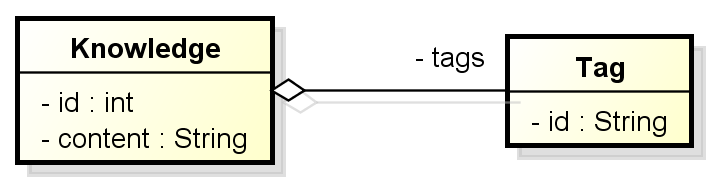
\includegraphics[width=5in]{img/uml}
	\caption{UML class-diagram of the model}
	\label{fig:uml}
\end{figure}

The main idea is to associate each \lstinline|Knowledge| object with a certain number of tags which can be searched for. This drastically reduces the amount of text to search, since only the tags (which are likely not that many) have to be compared. The rest is just very fast foreign-key matching.

\subsection{SOAP Message Structure}

SOAP (\textit{Simple Object Access Protocol}) is a networking protocol which uses XML to communicate. The message structure is defined in specific XML schema.

\begin{quote}
SOAP message is an ordinary XML document containing the following elements:

\begin{itemize}
	\item An Envelope element that identifies the XML document as a SOAP message
	\item A Header element that contains header information
	\item A Body element that contains call and response information
	\item A Fault element containing errors and status information
\end{itemize}
	
\begin{lstlisting}
<?xml version="1.0"?>
<soap:Envelope
xmlns:soap="http://www.w3.org/2001/12/soap-envelope"
soap:encodingStyle="http://www.w3.org/2001/12/soap-encoding">
	
<soap:Header>
...
</soap:Header>
	
<soap:Body>
...
<soap:Fault>
...
</soap:Fault>
</soap:Body>
	
</soap:Envelope>
\end{lstlisting}
\vspace{10pt}
\cite{soap}

\end{quote}

\section{Implementation}

\subsection{REST Webservice}

The REST Webservice was fully implemented within Python and using the Flask API,
especially using the Flask RESTful module. Below, we will show the esssential
part that was necessary for implementing a fully responsible RESTful API.  

The Webservice follows the design that was thoroughly described in section
\ref{sec:design}.

\subsubsection{URI}

The URI which can be used to call the different methods offered by the
webservice are listed down in the following table (Table \ref{tab:uri}).

\begin{table}[htbp]
  \centering
  \begin{tabular}{| c | c | c | l | } \hline
    \textbf{URI} & \textbf{Parameters} & \textbf{Method} & \textbf{Meaning} \\ \hline
    \lstinline|/q| & \lstinline|?tags=tag1,tag2| & \lstinline|GET| & Queries the data with the specified tags.  \\ \hline
    \lstinline|/knowledge| & \lstinline|content=str, tags=str| & \lstinline|POST| & Adds a new entry. \\ \hline
    \lstinline|/knowledge/<id>| &  & \lstinline|GET| & Retrieves the data of the given id  \\ \hline
    \lstinline|/knowledge/<id>| & \lstinline|content=str, tags=str| & \lstinline|PUT| & Updates the entry.   \\ \hline
    \lstinline|/knowledge/<id>| &  & \lstinline|DELETE| & Removes the entry with the given id \\ \hline
  \end{tabular}
  \caption{The URI options for the user}
  \label{tab:uri}
\end{table}

\subsubsection{Flask}

Two vital objects have to instantiated initially: 

\begin{lstlisting}
from flask import Flask
from flask.ext.restful import Api

app = Flask(__name__)
api = Api(app)
\end{lstlisting}
\vspace{10pt}

Now we need to define an API class for each resource that the webservice should
offer. These classes are required to implement the methods that are available,
e.g., GET, POST, PUT, ..., as Python methods with the same corresponding name,
however, in lowercase, e.g, get, put, post, etc. One example will be shown
below. 

\begin{lstlisting}
class KnowledgeAPI(Resource):
    def __init__(self):
        self.reqparse = reqparse.RequestParser()
        self.reqparse.add_argument('content', type=str)
        self.reqparse.add_argument('tags', type=str)

    def get(self, id):
        knowledge = Knowledge.query.filter_by(id=id).first()
        if knowledge is None:
            return {}
        return knowledge.mapped()

    def put(self, id):
        args = self.reqparse.parse_args()
        knowledge = Knowledge.query.filter_by(id=id).first()
        knowledge.content = args['content']
        knowledge.tags = [Tag(tag) for tag in args['tags'].split(',')]
        db.session.commit()
        return {'msg': 'Success'}

    def delete(self, id):
        knowledge = Knowledge.query.filter_by(id=id).first()
        db.session.delete(knowledge)
        db.session.commit()
        return {'msg': 'Success'}
\end{lstlisting}

\vspace{10pt}

The code is responsible for accessing the database with the elementary CRUD
commands. 

However, these classes must be added to the \lstinline|api| object first. 

\begin{lstlisting}
api.add_resource(KnowledgeQueryAPI, '/q')
\end{lstlisting}

\subsection{SOA Service}

The SOA part of this exercise was implemented with the help of \cite{jax-ws-example}.

\subsubsection{Service}

The step for creating a SOA service is to create an interface for the service.

\begin{lstlisting}
@WebService
@SOAPBinding(style = Style.RPC)
public interface IDontKnow {
	@WebMethod String query(String tag);
}
\end{lstlisting}

It is very important to add the correct annotations to mark this interface as a SOA service.
\\\\
This service-interface can then be implemented by a concrete service instance.

\begin{lstlisting}
@WebService(endpointInterface = "idontknow.IDontKnow")
public class IDontKnowImpl implements IDontKnow {

	@Override
	public String query(String tag) {
		System.out.println("Called `query()` with tag: \"" + tag + "\"");
	
		try {
			URL url = new URL("http://localhost:5000/q?tag=" + tag);
			URLConnection conn = url.openConnection();
			InputStream is = conn.getInputStream();

			return convertStreamToString(is);
		} catch(Exception e) {
			e.printStackTrace();
			return "Error: " + e.getMessage();
		}
	}
	...
}
 \end{lstlisting}
 
The only thing this our method implementation does, is to query the given Tag by calling our Rest-service.
\\\\
This implementation can then be published as real SOA webservice whith the code below.

\begin{lstlisting}
public class IDontKnowPublisher {
	public static void main(String[] args) {
		try {
			String url = "http://localhost:9999/ws/idontknow";
			Endpoint.publish(url, new IDontKnowImpl());
			System.out.println("Published `IDontKnowImpl` at \"" + url + "\"");
		} catch (Exception e) {
			e.printStackTrace();
		}
	}
}
\end{lstlisting}

It publishes an object of the service implementation at a specified URL. The Service is now running and can be accessed by clients via RPC.

\subsubsection{Client}

A SOA service can be accessed by many different clients. We implemented one in Java. To do that all that has creating a URL mapping it to the Service name and retrieving a remote  object of the service with \lstinline|service.getPort(IDontKno.class);| The methods of this retrieved instance can then be used similar to a local object. The full code is show below.

\begin{lstlisting}
public class IDontKnowClient {

	public static void main(String[] args) throws Exception {
		if (args.length != 1) {
			System.out.println("usage: IDontKnowClient <tag>");
			return;
		}

		try {
			URL url = new URL("http://localhost:9999/ws/idontknow?wsdl");
			QName qname = new QName("http://idontknow/", "IDontKnowImplService");

			Service service = Service.create(url, qname);
			IDontKnow idontknow = service.getPort(IDontKnow.class);

			System.out.println(idontknow.query(args[0]));
		} catch (Exception e) {
			System.out.println("Something went wrong: " + e.getMessage());
		}
	}

}
\end{lstlisting}

\subsubsection{WSDL}

A proper WSDL file is automatically generated when the service is published and is available at the given URL. So we opened \lstinline|http://localhost:9999/ws/idontknow?wsdl| and saved the response in a simple XML-file which is also shown below. The file is shipped with the submission in the \lstinline|wsdl.xml| file.

\begin{lstlisting}

\end{lstlisting}

\section{Testing}

Tests with small a dataset were performed. 

\subsection{Creating the Schema}

\begin{figure}[h!]
  \centering
  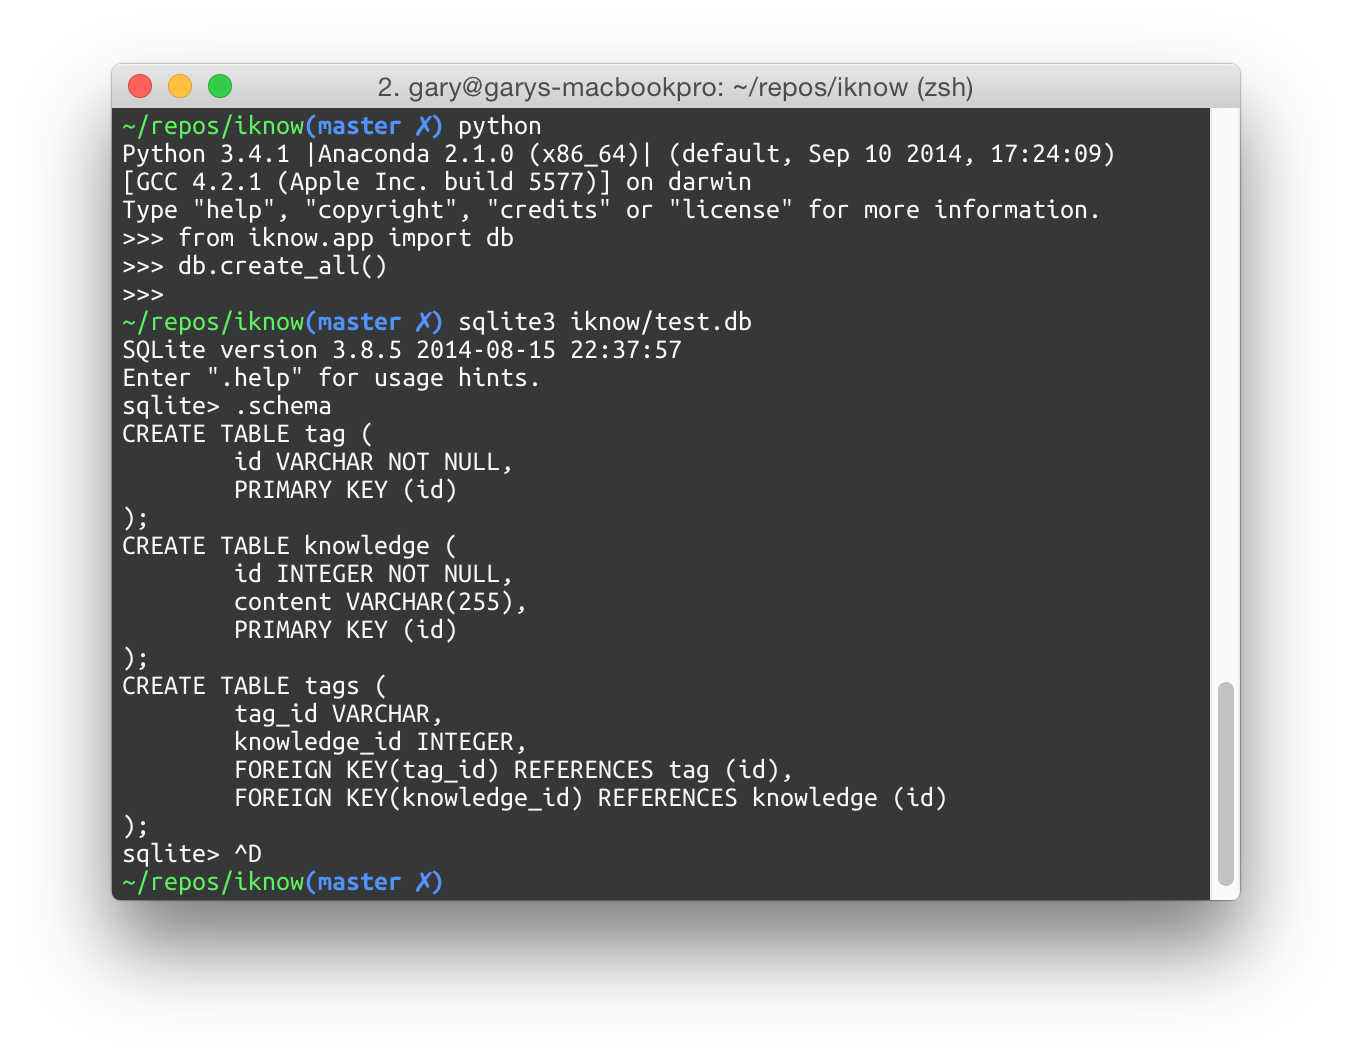
\includegraphics[width=0.7\textwidth]{img/schema}
\end{figure}

\begin{figure}[h!]
  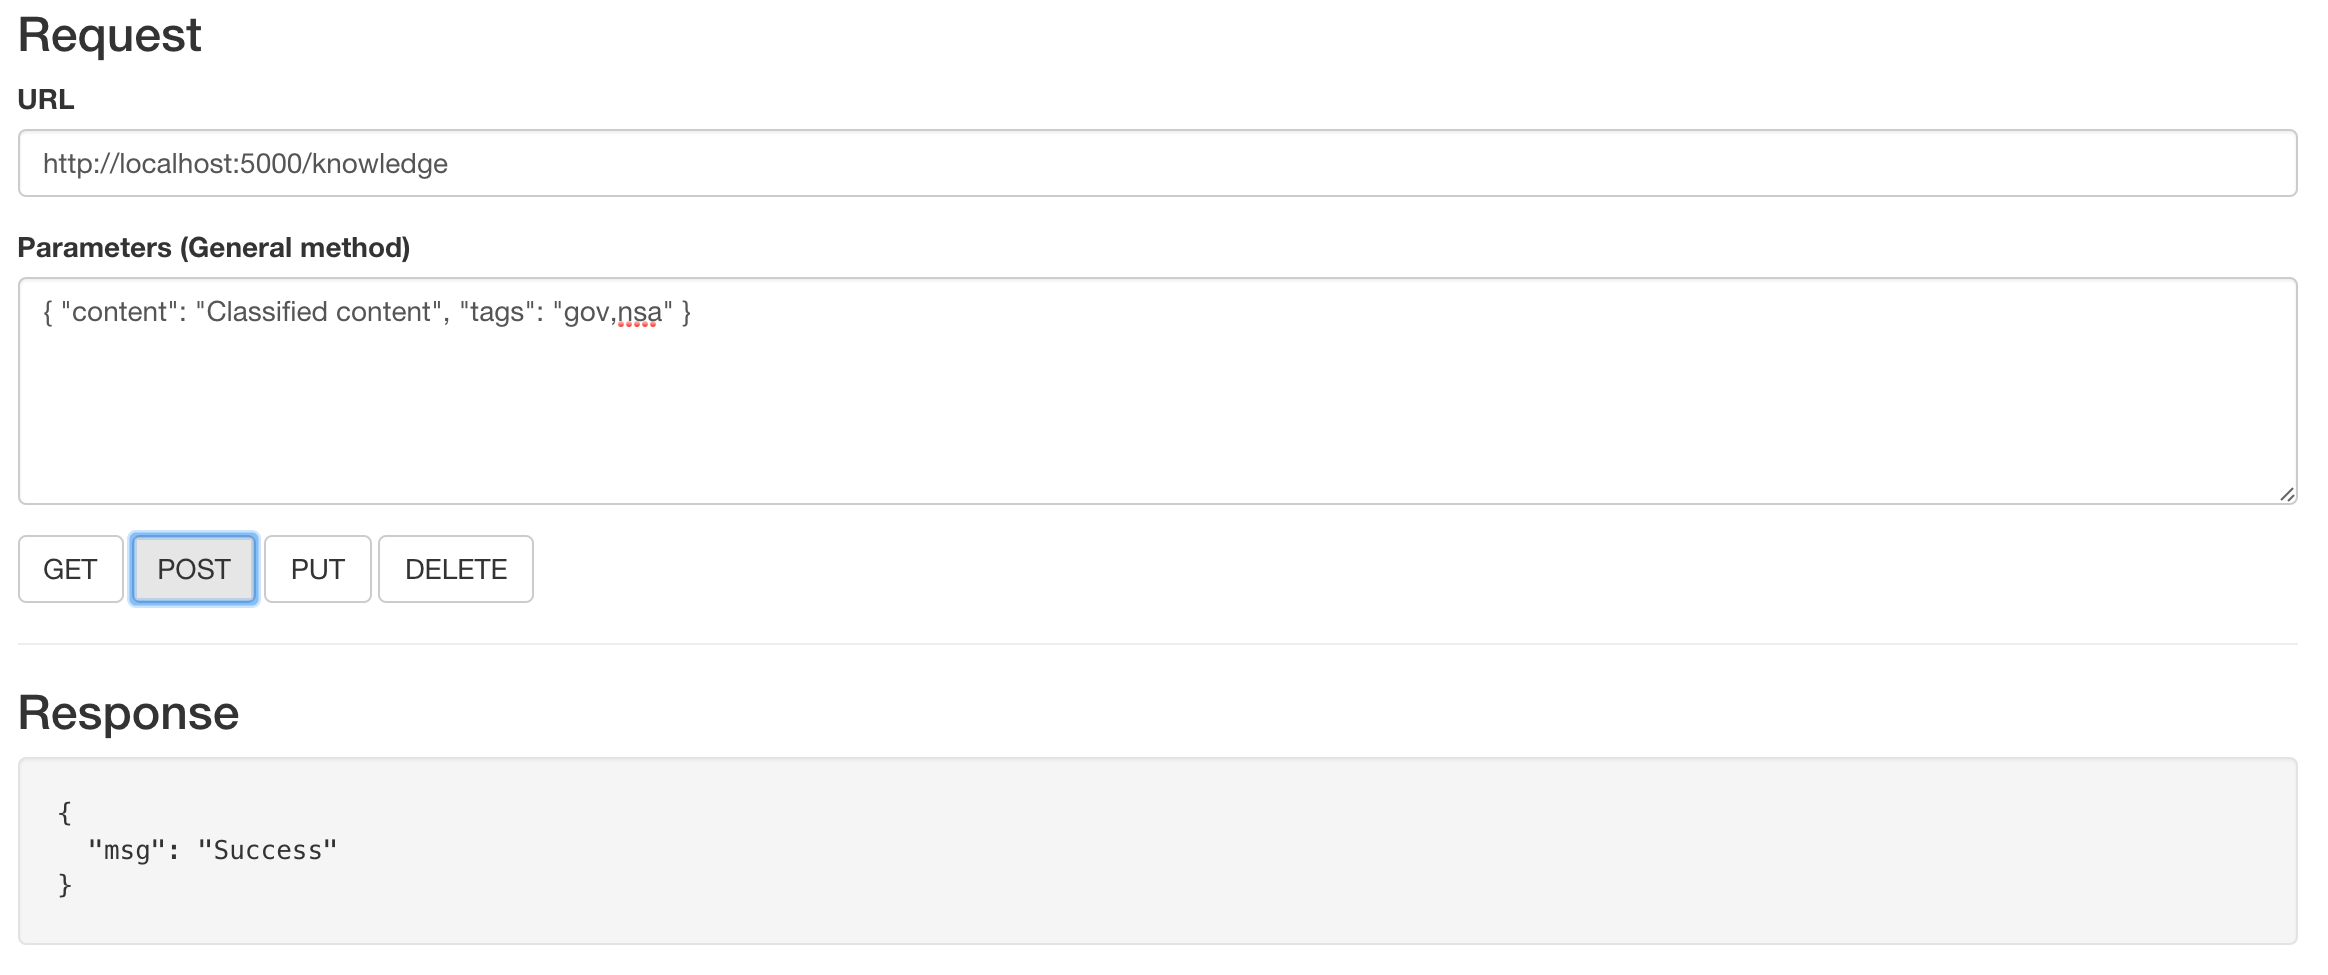
\includegraphics[width=\textwidth]{img/testput0}
\end{figure}

\begin{figure}[h!]
  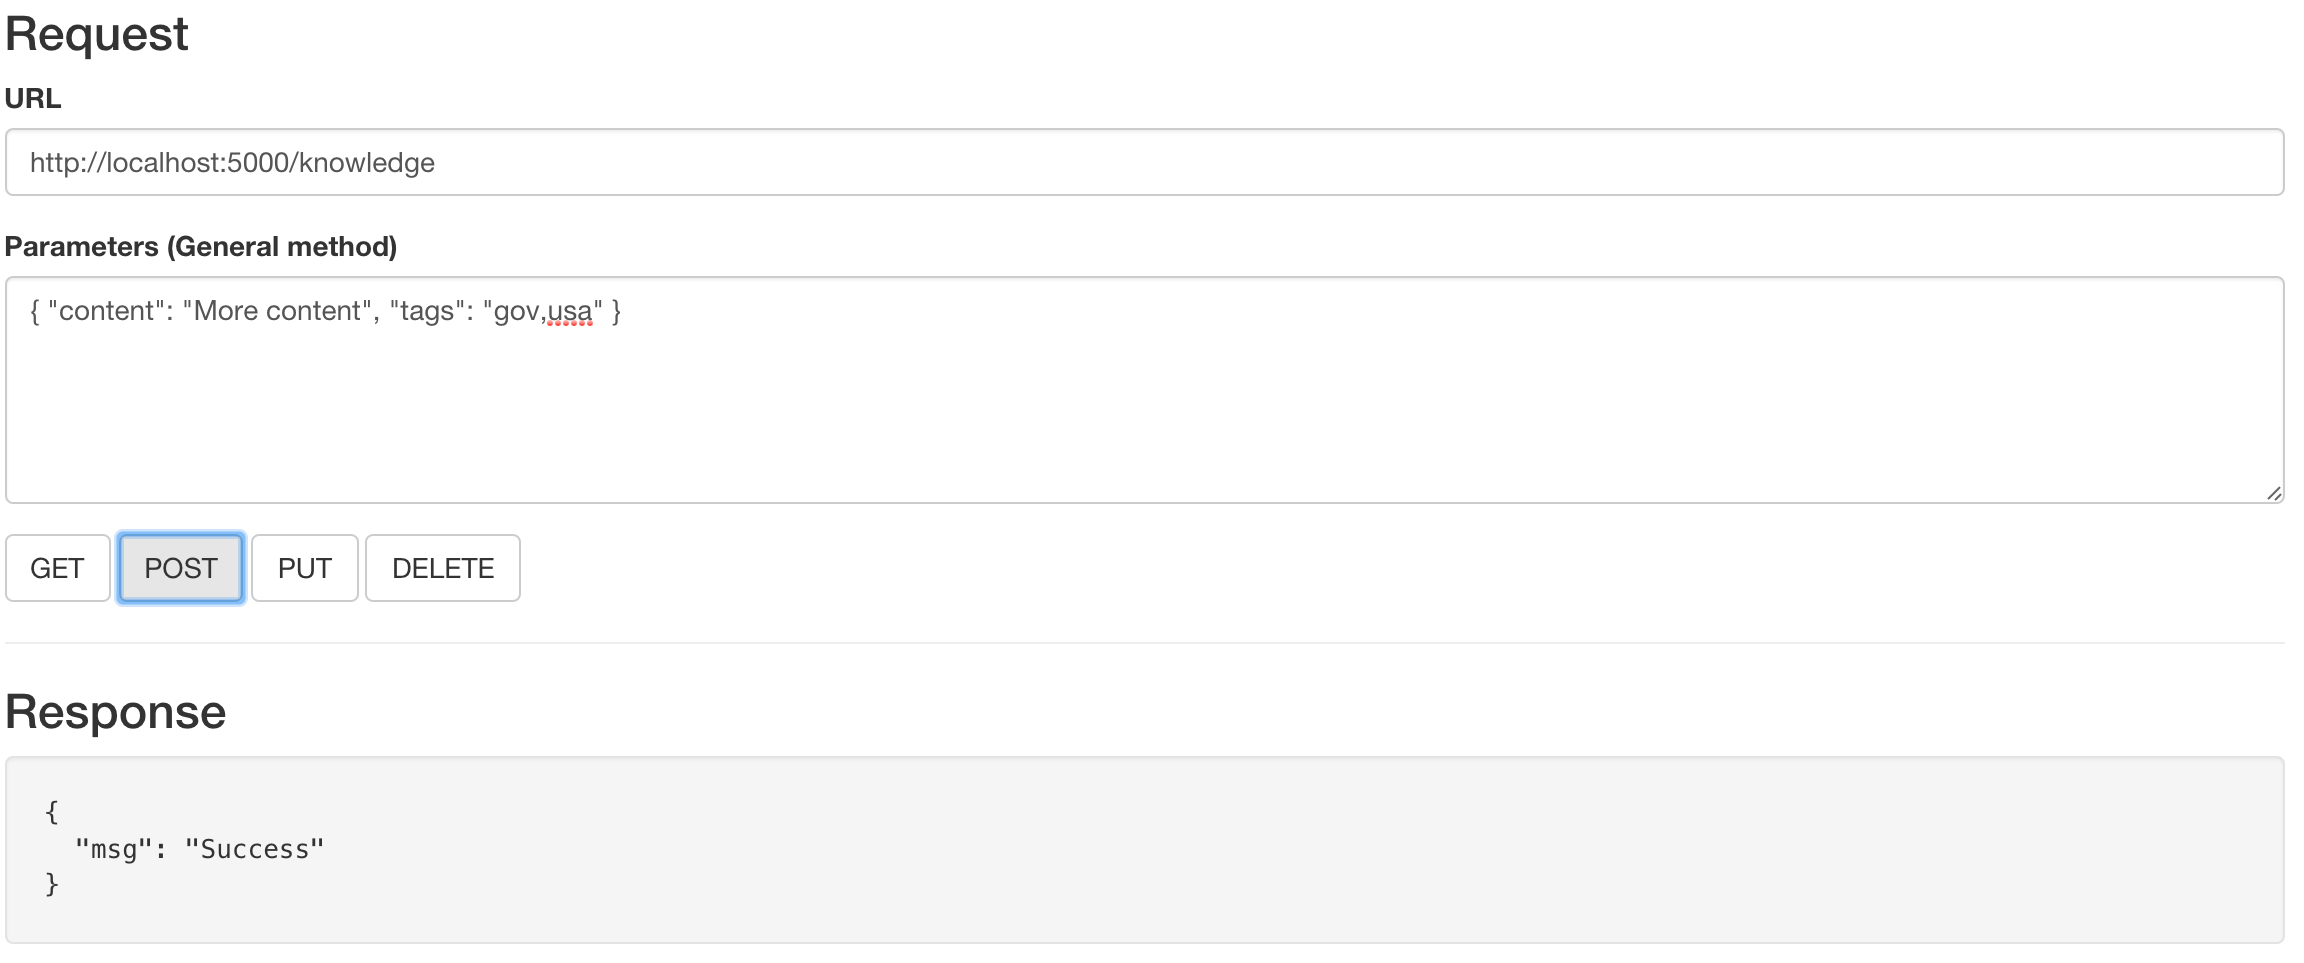
\includegraphics[width=\textwidth]{img/testput1}
\end{figure}

\section{Problems \& Solutions}

No major problems occurred while realizing this exercise.

\nocite{*}
\bibliographystyle{plain}
\bibliography{bibliography}

\end{document}
